% REVIEW-CANDIDATE. Independent report audit and user submission approval pending.
% Authoritative requirements: ../local-materials/midproject-assignment.json.
% Scientific evidence: final-training-review.json and final-results-review.json (PASS).
% Do not modify the frozen experiment source, configs, tests, or README.
% Compile with scripts/build_report.sh. Prior DRAFT snapshots remain preserved.
\documentclass[journal]{IEEEtai}
\usepackage{amsmath}
\usepackage{array}
\usepackage{graphicx}
\usepackage{cite}
\usepackage[hidelinks]{hyperref}
\newcommand{\pending}[1]{\par\noindent\textbf{PENDING:} #1\par}

\begin{document}
\title{Learning When to Recheck: Cost-Aware Reinforcement Learning for Navigation with Stale Maps}
\author{Essam Benamar, Khush Birjoo Mistry, and Sandipsinh Rathod%
\thanks{COMP 597 course project, November 7, 2026. Review candidate, not submitted. Independent report audit remains pending.}}
\markboth{COMP 597 Mid-Project Report: Review Candidate, November 7, 2026}{Benamar, Mistry, and Rathod: Learning When to Recheck}
\IEEEspecialpapernotice{REVIEW-CANDIDATE: independent report audit pending}
\maketitle

\begin{abstract}
Remembered routes can become unreliable when passage states change, but inspecting every passage also costs time. We investigate selective physical reinspection using a graph surrogate with persistent beliefs and a travel budget. This is not an Unreal Engine experiment. Full-feature and masked-feature policies were trained with proximal policy optimization using five seeds each and 98,304 decisions per run. Evaluation used 128 held-out six-task sequences per regime across three regimes, with reactive, age-based, memory-reset, and value-of-information baselines. Both learned variants and value-of-information planning achieved 100\% observed success without inspections and matched the safe-route cost on every evaluated task. Thus the study does not demonstrate learned reinspection, an explicit-feature benefit, or an advantage over value-of-information planning. Failure avoidance lowered penalized cost in changing regimes but increased raw travel time. The static paired interval includes zero. The contribution is a controlled negative result that motivates stronger action-discriminating benchmarks, not a claim of general navigation superiority.
\end{abstract}

\section{Introduction}
A navigation agent can remember that a passage was open without knowing whether it remains open. Trusting stale observations can waste travel and exhaust a task budget. Reinspection can prevent late discovery, but it also requires movement and sensing time. Useful decisions must consider uncertainty, route alternatives, and the consequences of failure.

Reinforcement learning (RL) is suitable because an inspection changes the information available for later decisions and tasks. Our research question is whether a task-conditioned reinspection policy improves the success--cost trade-off over tuned classical alternatives. We hypothesized that explicit memory-age and route-cost features would help select useful inspections. A successful navigation outcome alone does not confirm this mechanism.

The Canadian Traveler Problem with Remote Sensing already combines travel and information costs~\cite{Bnaya2009CTPSensing}. D* Lite addresses replanning after new evidence~\cite{Koenig2002DStarLite}. Our proposed distinction is physically costly reinspection of persistent route memory, not the invention of sensing or replanning.

The September proposal planned an Unreal Engine building environment. The implemented first stage is a parallel-corridor graph surrogate. It isolates decision logic but omits rendering, visibility geometry, and low-level control. An independent implementation gate passed after 164 acceptance tests and 259 boundary probes. Subsequent training and results audits verified saved evidence, but did not independently replay navigation. This report remains a review candidate.

The intended contributions are:
\begin{enumerate}
\item A controlled graph experiment that separates passage changes, missed inspections, and physical inspection costs.
\item A matched full-versus-masked RL comparison against reactive, age-based, reset, and sensing-aware controls.
\item Evidence about the tested mechanism, including the present negative result: reliable safe-route behavior does not establish useful learned reinspection.
\end{enumerate}

\section{Related Work}
\subsection{Cost-aware sensing and replanning}
Bnaya et al. study travel and sensing in the Canadian Traveler Problem~\cite{Bnaya2009CTPSensing}. Their single-step value-of-information (VOI) policy is a close predecessor. Its remote sensing operation differs from moving an agent to an inspection viewpoint. Our adaptation enumerates eight door-state worlds and charges travel and sensing costs. It is not an exact reproduction of their system.

D* Lite reuses search information as edge costs change~\cite{Koenig2002DStarLite}. Receiving a new edge cost differs from deciding whether to pay to observe it. Our reactive control chooses the lowest-cost eligible corridor or safe route. It does not implement D* Lite and is not labeled as such.

\subsection{Temporal prediction and persistent memory}
FreMEn models temporal regularity and recent-state persistence~\cite{Krajnik2017FreMEn}. It establishes that age-sensitive prediction is not new. Our experiment supplies known independent flip probabilities instead of fitting a temporal model. It neither implements nor reproduces FreMEn.

GOAT-Bench studies navigation sequences with explicit and implicit memory~\cite{Khanna_2024_CVPR}. MemoNav uses working-memory representations and selective forgetting~\cite{Li_2024_CVPR}. These works motivate cross-task memory, but relevance and physical validity differ. A passage can remain relevant while its remembered state becomes unreliable. 3D-Mem combines scene memory with frontier information for exploration~\cite{Yang_2025_CVPR}. Our setting instead revisits known structure with uncertain traversability. These visual-navigation systems provide context, not directly comparable benchmark scores.

\subsection{Stale information and active perception}
The EvoNav-Bench preprint studies navigation after object relocations and compares reactive updates with memory resets~\cite{Wang2026EvoNav}. Its changes preserve room topology. Our graph changes passage traversability while retaining a safe route, but cannot support conclusions about evolving visual scenes.

SPIN coordinates perception, interaction, and navigation~\cite{Uppal_2024_CVPR}. Malczyk et al. learn aerial motion and camera control~\cite{Malczyk2026ActivePerception}. Both establish observation acquisition as a learned decision. Our fixed travel model does not reproduce their perception or motor-control systems. The Malczyk citation identifies the inspected preprint and author-reported acceptance, not a separately verified proceedings version.

\subsection{Optimization and positioning}
Proximal policy optimization (PPO) supplies the policy-update algorithm~\cite{Schulman2017PPO}; it is not the novelty. The full and masked variants share architecture, optimizer, seeds, and budget. These ten papers motivate a bounded mechanism test, not an exhaustive novelty claim. Our negative result shows why a reliable policy must not automatically be described as a learned sensing policy.

\section{Problem Formulation}
\subsection{State and partial observability}
The underlying Markov decision process has state
\begin{equation}
s_t=(L,x_t,D_t,h_t,B_t,k_t),
\end{equation}
where $L$ contains layout costs and regime parameters, $x_t$ is position, and $D_t$ contains three hidden binary door states. Public memory $h_t$ records legitimate evidence and its age; $B_t$ is remaining budget; $k_t$ is the task index. An episode contains six tasks. Positive travel and sensing costs and finite budgets bound the decisions.

The agent cannot observe $D_t$. It receives position, budget, task index, beliefs, last observations, known-state flags, boundary ages, and current-task observation and inspection-attempt flags. Costs and known flip/miss probabilities are public. Hidden state and seed identifiers are excluded from both actor and critic. The agent therefore faces a partially observable process, with an exact belief-state representation under the supplied model. Unequal action durations are charged through reward.

\subsection{Actions and transitions}
The seven legal actions are three shortcut choices $\mathrm{TAKE}_i$, three inspections $\mathrm{INSPECT}_i$, and $\mathrm{TAKE\_SAFE}$. Each action routes through hub $S$, even after a repeated choice. A shortcut travels to approach $U_i$ and observes the door on completed arrival. An open door permits crossing to goal $G$; a blockage leaves the agent at $U_i$. Later actions pay return travel.

Inspection travels to viewpoint $V_i$ and pays sensing time. It reveals only its selected door and can miss. There is no incidental visibility. An interrupted action consumes only the remaining budget and cannot reveal evidence from an unreached event. Exact-budget events precede timeout; floating-point equality uses a four-unit-in-the-last-place tolerance with residuals clamped to zero.

Doors stay fixed within a task and can flip independently at boundaries. Intermediate success or failure resets position and budget to $S$ while preserving memory. This is an exogenous reset, not simulated return travel. For open belief $q_i$ and known flip probability $p$,
\begin{equation}
q'_i=(1-p)q_i+p(1-q_i).
\end{equation}
Missing evidence leaves the belief unchanged. The final task ends the sequence without another transition.

\subsection{Reward and objective}
For consumed graph time $\Delta t$, raw reward is
\begin{equation}
r_t=-\Delta t+100\mathbf{1}_{\mathrm{success}}-100\mathbf{1}_{\mathrm{failure}}.
\end{equation}
The time penalty charges sensing and movement. Task payouts discourage cheap but unsuccessful behavior. Six-task return is $600-T_{\mathrm{seq}}-200F$, where $F$ counts failures. Maximizing return therefore minimizes time plus 200 per failure, not time alone.

The finite sequence objective uses $\gamma=1$. PPO scales rewards once by $0.01$. Generalized advantage estimation (GAE) uses $\lambda=0.95$ per decision, not per time unit. Intermediate task boundaries do not terminate GAE. Rollout cuts bootstrap; sequence endings do not. No continuous-time discount modification is claimed.

\section{Planned Method}
\subsection{Implemented policy and update procedure}
The graph prototype implements PPO in PyTorch. Separate actor and critic networks each have two 64-unit tanh layers and the same 42-dimensional input. The actor outputs seven categorical-action logits; the critic outputs one value. Weights use orthogonal initialization and zero biases. Hidden-layer gain is $\sqrt{2}$; actor and critic output gains are $0.01$ and $1$.

The masked variant zeros 15 explicit columns: three boundary ages, three approach costs, three crossing costs, three viewpoint costs, sensing cost, safe-route cost, and initial budget. Vector size, position, current budget, task index, public memory, and known regime parameters are unchanged. Beliefs and budget retain indirect age/cost information. This is not removal of all temporal or cost information.

\begin{quote}
\textbf{Implemented sequence-training procedure}
\begin{enumerate}
\item Cycle regimes at sequence creation; draw layout and world trajectory from separate random streams.
\item Encode public observations with fixed scaling and the selected feature mask.
\item Sample a categorical action; charge physical time and record only reached observations.
\item At intermediate outcomes, retain evidence, propagate beliefs once, and reset position and budget.
\item Collect a rollout, scale rewards, and compute decision-step GAE with $\gamma=1$ and $\lambda=0.95$.
\item Normalize advantages across the batch and apply clipped PPO updates. Save the final-budget checkpoint and logs.
\end{enumerate}
\end{quote}

\subsection{Sensing-aware control and limitations}
VOI evaluates all seven first actions over eight possible door worlds weighted by public beliefs. It includes sensing misses, position, budget, and failure penalties. Each first action is followed by reactive navigation that receives only physically encountered evidence, with no further simulated inspection. After one real action, VOI replans. This is exact expectation for a restricted continuation, not optimal partially observable planning.

\textbf{Horizon mismatch:} VOI stops at the current task; PPO optimizes the six-task sequence. Their horizons differ even though they use the same undiscounted task-cost ranking. A performance difference would not isolate better matched-horizon sensing. The current data show no advantage over VOI.

The implemented choices are frozen. Whether fitted models, less restricted topology, or different task distributions change the conclusion is undecided and belongs to a prospective study. No held-out result was used to retune the current experiment.

\section{Environment and Data}
\subsection{Graph-only environment}
The environment is \texttt{stale-nav} version 0.1.0: three shortcuts and one always-open route. Source and configuration SHA256 digests identify the frozen implementation. It was chosen to isolate sensing and belief contracts before rendering integration. Graph time is abstract travel/sensing cost, not Unreal seconds. The proposed Unreal rooms, blockers, visibility, and low-level controller remain future work. There are no Unreal or real-world results here.

Layout draws are uniform: safe-route cost in $[20,30]$, approach costs in $[6,14]$, crossing costs in $[1,4]$, viewpoint costs in $[0.5,2.5]$, and sensing time in $[0.5,2]$. Budget is safe-route cost times a factor in $[1.1,1.6]$. The safe route is therefore always feasible at task start. Initial open probability is $0.5$.

Training cycles regimes equally at sequence creation: static clean $(p,m)=(0,0)$, changing clean $(0.2,0)$, and changing with misses $(0.2,0.25)$. Regime and layout stay fixed within each sequence; $m$ is inspection-miss probability. Different policy durations can yield different completed-sequence counts under an equal decision budget.

\subsection{Data and preprocessing}
Experience comes from interaction, not offline or language-model training data. The encoder uses 42 float32 features and fixed analytic scales, never fitted test statistics. Position has eight one-hot entries. Budget scale is 48, task/age scale is 5, and cost scales follow their known upper bounds. Unknown observations have separate known-state flags. There is no image preprocessing or external environment wrapper. Sixteen environment instances step in a Python loop while model operations use batches.

Training, validation, test, and pilot IDs have disjoint namespaces. Layout and world streams are separate. Sensing misses are keyed by scenario, task, door, and that door's attempt number, so unrelated action counts cannot shift the world. The exact independent transition model is supplied, not fitted. Known parameters, forced hub routing, repeated-origin resets, and one fixed topology limit generalization.

\section{Experimental Setup}
\subsection{Baselines and validation}
Reactive navigation chooses the lowest-cost route not remembered blocked, including the safe route. Memory reset retains current-task evidence but discards prior-task state history. Route-conditioned time-to-live (TTL) inspects a previously observed door only when reactive routing selects it, its age reaches $k$, and that door has not been inspected this task. A miss consumes the attempt. Remembered-blocked doors are never selected, so TTL does not proactively discover reopened passages.

TTL selection tested $k\in\{1,2,3,6\}$ on the same 64 validation sequences per regime and threshold. It minimizes mean sequence penalized cost, with smaller-threshold ties. Independent review confirmed $k=2$ for static clean and $k=1$ for both changing regimes. These choices were frozen before test evaluation. VOI and the two PPO variants complete the six-policy comparison; no privileged oracle is included.

\subsection{Training configuration and compute}
All ten final runs completed: five seeds $\{0,1,2,3,4\}$ for each PPO variant, each with 98,304 environment decisions. Independent training review verified the saved logs, finite parameters and optimizer state, checkpoint budgets, and matching source/configuration hashes. Table~\ref{tab:config} lists the shared settings.

\begin{table}[t]
\caption{Frozen PPO configuration, shared by both variants.}
\label{tab:config}\centering\small
\begin{tabular}{lr}\hline
Parameter & Value \\ \hline
Hidden layers; activation & $64,64$; tanh \\
Environment instances; rollout length & $16$; $128$ \\
Epochs; minibatch size & $4$; $256$ \\
Learning rate; Adam epsilon & $0.0003$; $10^{-5}$ \\
Clip; entropy coefficient & $0.2$; $0.01$ \\
Value coefficient; gradient norm cap & $0.5$; $0.5$ \\
Discount; decision-step GAE & $1$; $0.95$ \\
Training reward scale & $0.01$ \\
Steps/run; training seeds/variant & $98{,}304$; $5$ \\ \hline
\end{tabular}
\end{table}

The first cold 4,096-step pilot projected 116.7 minutes for ten original-budget runs, exceeding the predeclared 90-minute rule. Both variants therefore used the half-budget fallback while retaining all five seeds. Later warm speedup did not reverse this conservative pre-test choice. Checkpoints were selected by completed budget, not test score.

% Generated from the PASS training audit and evaluation runtime provenance.
Training used CUDA on an NVIDIA GeForce RTX 5090, with PyTorch 2.8.0+cu128, Python 3.12.16, and NumPy 2.5.4. The ten recorded training-loop times sum to 87.453875 seconds; individual loops range from 8.610 to 9.202 seconds. These timers include rollout collection, PPO updates, and in-loop logging. They exclude initial provenance creation, model/optimizer setup, and initial environment construction, as well as final checkpoint and artifact serialization. They are not end-to-end process timings or evidence of real-time navigation. No independently captured batch process timer or separate inference-latency measurement is claimed.


\subsection{Evaluation and uncertainty}
Evaluation uses deterministic highest-logit PPO actions and 128 held-out six-task sequences per regime. Four classical policies and ten trained models produce 5,376 sequence rows and 32,256 task rows across three regimes. All policy/model instances share scenario IDs. Saved world/layout hashes, split separation, pairing, and task-to-sequence identities passed independent checks.

Primary metrics are success, all-task graph time, inspections, blocked attempts, raw reward, and penalized cost. Time includes failures. An inspection is counted when selected, even if budget exhaustion prevents sensing. Per-task penalized cost is $C=T+200(1-S)$ for success fraction $S$; mean raw reward is $100-C$.

Training-seed standard deviation (SD) is separate from sequence uncertainty. Paired contrasts average models within each scenario and then subtract reactive performance on that scenario. Normal 95\% intervals use 128 paired sequences and are conditional on the five models. The seed-by-sequence product is not an independent sample. Intervals are exploratory and unadjusted for multiple comparisons.

\section{Preliminary Results}
% Generated from audited CSVs by report/generate_results.py.
\begin{table*}[t]
\caption{Held-out graph results. Each regime uses 128 paired six-task sequences. PPO entries average five independently trained models; classical policies have one deterministic instance. $T$: failure-inclusive graph time/task; $I$: inspection attempts/task; $B$: blocked attempts/task; $C=T+200(1-S/100)$: penalized cost/task. Cost SD is across the five model means, not sequence uncertainty.}
\label{tab:results}\centering\small
\begin{tabular}{llrrrrrr}\hline
Regime & Policy & $S$ (\%) & $T$ & $I$ & $B$ & $C$ & Cost seed SD \\ \hline
Static clean & Reactive & 93.49 & 14.57 & 0.000 & 0.138 & 27.60 & n/a \\
 & Route-conditioned TTL & 93.49 & 14.57 & 0.000 & 0.138 & 27.60 & n/a \\
 & Memory reset & 71.09 & 21.20 & 0.000 & 0.727 & 79.01 & n/a \\
 & VOI & 100.00 & 25.55 & 0.000 & 0.000 & 25.55 & n/a \\
 & Full PPO & 100.00 & 25.55 & 0.000 & 0.000 & 25.55 & 0.00 \\
 & Masked PPO & 100.00 & 25.55 & 0.000 & 0.000 & 25.55 & 0.00 \\
\hline
Changing clean & Reactive & 82.03 & 18.68 & 0.000 & 0.316 & 54.62 & n/a \\
 & Route-conditioned TTL & 87.63 & 19.90 & 0.595 & 0.201 & 44.64 & n/a \\
 & Memory reset & 67.71 & 20.75 & 0.000 & 0.720 & 85.33 & n/a \\
 & VOI & 100.00 & 24.77 & 0.000 & 0.000 & 24.77 & n/a \\
 & Full PPO & 100.00 & 24.77 & 0.000 & 0.000 & 24.77 & 0.00 \\
 & Masked PPO & 100.00 & 24.77 & 0.000 & 0.000 & 24.77 & 0.00 \\
\hline
Changing with misses & Reactive & 80.60 & 19.02 & 0.000 & 0.326 & 57.82 & n/a \\
 & Route-conditioned TTL & 84.24 & 20.62 & 0.561 & 0.253 & 52.13 & n/a \\
 & Memory reset & 70.96 & 20.38 & 0.000 & 0.715 & 78.45 & n/a \\
 & VOI & 100.00 & 24.87 & 0.000 & 0.000 & 24.87 & n/a \\
 & Full PPO & 100.00 & 24.87 & 0.000 & 0.000 & 24.87 & 0.00 \\
 & Masked PPO & 100.00 & 24.87 & 0.000 & 0.000 & 24.87 & 0.00 \\
\hline
\end{tabular}
\end{table*}

% Generated from paired_differences.csv; sequence costs divided by six.
\begin{table}[t]
\caption{Full PPO minus reactive penalized cost per task. Negative differences favor PPO on this penalized metric, not raw time. Intervals use 128 paired sequences per regime, conditional on the five models, and are exploratory and unadjusted.}
\label{tab:paired}\centering\small
\begin{tabular}{lrr}\hline Regime & Mean & Normal 95\% CI \\ \hline
Static clean & $-2.04$ & $[-6.81, 2.73]$ \\
Changing clean & $-29.84$ & $[-36.28, -23.41]$ \\
Changing with misses & $-32.95$ & $[-39.41, -26.49]$ \\
\hline\end{tabular}
\end{table}

% Verified aggregate PNG and its CSV inputs are recorded in results-manifest.json.
\begin{figure}[t]
\centering
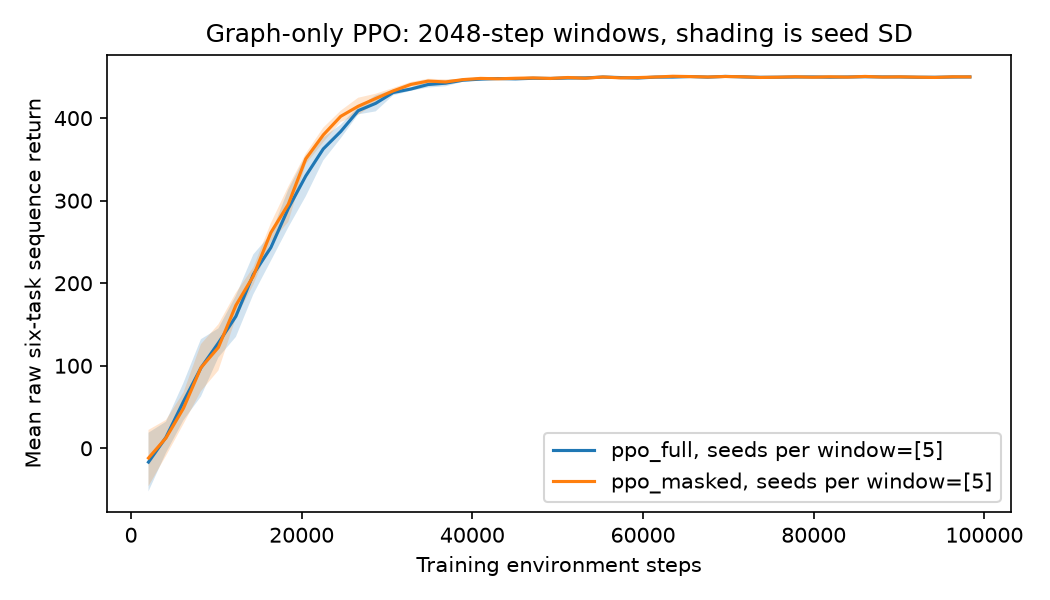
\includegraphics[width=\columnwidth]{generated/learning_curve.png}
\caption{Graph-only PPO training. Each point averages five independent seeds; shading is $\pm1$ sample standard deviation of seed means, not a confidence interval over held-out sequences. Fixed 2,048-step windows use completed raw six-task sequence returns, ending at 98,304 steps. There are 48 points per variant, 96 total. Partial trailing sequences are excluded. Improved return does not demonstrate learned inspection.}
\label{fig:learning}
\end{figure}


\subsection{Reliable navigation without learned inspection}
Table~\ref{tab:results} shows the main negative result. Full PPO, masked PPO, and VOI have identical saved outcomes on every held-out scenario, not merely matching means. Each achieves 100\% observed success with zero inspection and blocked attempts. All 25,344 task records for these 11 policy/model instances match their scenario's deterministic safe-route cost.

Under the frozen action semantics, these records imply safe-route navigation. Evaluation did not save a per-action trace, so the conclusion comes from recorded outcomes and the cost model, not a replayed action log. Neither PPO variant demonstrates selective reinspection. Full PPO does not outperform VOI, and masking explicit age/cost features changes no held-out outcome. This is a negative result for the intended mechanism, not evidence that these features can never help.

The reliability gain relative to reactive navigation comes with slower travel. In changing clean scenarios, full PPO takes 24.77 time units/task versus reactive's 18.68, while penalized cost is 24.77 versus 54.62. With misses, the corresponding times are 24.87 versus 19.02, and costs are 24.87 versus 57.82. These cost differences reflect failure avoidance, not faster routes or a sensing advantage.

\subsection{Baselines, contrasts, and variability}
TTL raises changing-clean success from 82.03\% to 87.63\% and changing-missed success from 80.60\% to 84.24\%. It adds inspections and elapsed time. Static TTL matches reactive exactly. Memory reset has lower observed success and higher penalized cost than reactive in every regime, consistent with losing useful route history in this setting.

Table~\ref{tab:paired} separates sampling uncertainty from training-seed variation. Static full-minus-reactive cost is $-2.04$ per task with interval $[-6.81,2.73]$, which includes zero. Changing-regime intervals lie below zero on the penalized metric. We do not claim universal superiority. Full-minus-VOI and full-minus-masked differences are zero on every saved scenario. Zero empirical variation is not proof of population equivalence or zero future failure risk.

Figure~\ref{fig:learning} contains 96 independently recomputed curve points, each based on five seed means. Full PPO's mean raw sequence return rises from $-16.76$ to $449.89$; masked PPO rises from $-11.86$ to $449.91$. Their final-window seed SDs are $0.364$ and $0.392$. The curves measure stochastic training, whereas held-out actions are deterministic. Nonzero training-curve variation therefore coexists with identical final held-out behavior.

No failed or nonfinite final training run was found in the audited ten-run package. This execution success does not rescue the mechanism hypothesis. Earlier implementation reviews found budget-equality and numerical tie defects; these were corrected before the final source freeze and rechecked by the 164 tests and 259 independent probes. Earlier blocked audits and pilot evidence remain preserved rather than being presented as final results.

\section{Discussion}
The experiment shows reliable conservative navigation, not learned selective reinspection. The guaranteed safe route, tested budgets, and failure penalty plausibly favor that behavior. This explains why higher return can occur without sensing, but does not prove global optimality. Success with missed observations also does not demonstrate learned tolerance of sensing failures: PPO and VOI never inspect.

The full/masked equality gives no evidence that the added explicit features improved this benchmark. Beliefs and remaining budget still carry indirect age/cost information, so the ablation cannot establish that temporal or cost information is irrelevant. Likewise, the sequence-trained PPO and task-myopic VOI horizons remain mismatched despite their identical measured outcomes.

The scope changed from planned Unreal navigation to a graph-only mechanism test. Known transition probabilities replace the proposal's fitted model; resets omit return travel between tasks; forced hub routing and absent incidental visibility simplify geometry. Five seeds, one topology, deterministic evaluation, and 128 sequences/regime limit external validity. Independent results review recomputed saved statistics and scenario construction, but did not conduct a new navigation replay.

The useful outcome is a benchmark-design diagnosis. A high success score and an improving learning curve are insufficient to establish the proposed sensing mechanism. Raw time, failure-inclusive cost, inspection counts, the strong VOI baseline, and the feature ablation must be interpreted together.

\section{Remaining Plan and Risks}
The current experiment is frozen. No further tuning on its held-out results is planned. The main scientific risk is repeating a task distribution that rewards safe-route behavior without testing when information acquisition matters.

\begin{itemize}
\item \textbf{November 7--8:} complete independent report audit, check the 4--6-page body limit, and reconcile the candidate with the accepted evidence. The current mid-project deadline is November 8 at 11:59 p.m. Eastern, not the proposal's tentative November 3 date.
\item \textbf{November 9--22:} preregister a new study with an explicit ALWAYS-SAFE comparator and held-out cases where direct travel, inspection, and safe routing each have an advantage. Validate those cases analytically before training; do not retrofit the current test set.
\item \textbf{November 23--December 1:} assess matched-horizon sensing controls, fitted transition models, and tested Unreal integration as separate extensions. Preserve the current graph result regardless of their outcome.
\item \textbf{December 2--15:} consolidate evidence and revise the final report. The proposal's December 8 presentation and December 15 report dates remain tentative until current course requirements are confirmed.
\end{itemize}

The fallback is a rigorous negative-result report with reproducible classical comparisons, not an unsupported claim that RL must win. Team ownership is not assigned here.

\section*{Code Availability}
A local reproducibility package contains the graph source, tests, configurations, README, execution helpers, immutable source archives, and raw-data aggregation. Experiment files remain hash-frozen; the README retains historical progress statements until that freeze ends. Current status is established by the dated approval and run records, not those historical sentences.

\pending{GitHub link and instructor access are deferred by user decision to authorize local Git only. No public repository or access grant is claimed. This assignment requirement remains unmet.}

Report tables and the figure are generated under \texttt{report/generated/}. The report-only generator verifies input CSV hashes against the independent results audit, recomputes statistics, and records output hashes. Source-paper PDFs, private course exports, caches, and credentials remain outside Git. This review candidate is not a submitted or independently report-audited document.

\noindent\textbf{Tool-assistance disclosure.}
Forge, an OpenAI AI assistant, assisted with reviewing supplied course materials, literature records, frozen code, and audit evidence; drafting prose; deriving tables; and LaTeX/PDF build checks. Bibliographic descriptions use the supplied curated catalog rather than reproducing the cited systems. AI assistance is not experimental evidence. The authors must review the report and its claims before submission; no individual team contributions are inferred from tool use.

\label{report-body-end}
\clearpage
\bibliographystyle{IEEEtran}
\bibliography{references}
\end{document}
